\chapter{Fundamentação teórica}\label{cap:teoria}

Neste capítulo são apresentados os conceitos em que o trabalho se apoia: o princípio da síntese digital direta e suas fontes de erro; os dispositivos lógicos programáveis, a linguagem \ac{vhdl} e o acesso por \ac{jtag}; e os circuitos analógicos que convertem as amostras digitais em tensão. O leitor interessado pode aprofundar os conceitos através das referências.

\section{Síntese digital direta}

A \ac{dds} gera um sinal periódico a partir de um clock de referência de frequência fixa, \(f_{clk}\). A arquitetura clássica, mostrada na Figura~\ref{fig:dds_blocos}, tem quatro blocos: um acumulador de fase de \(N\)~bits, que avança um passo \(M\) a cada clock; um truncamento, que aproveita apenas os \(P\)~bits mais significativos da fase; uma \ac{lut}, que converte a fase em amplitude com \(D\)~bits; e um \ac{dac} seguido de um filtro passa-baixas, que reconstroem o sinal analógico \cites{tierney1971,ad1999,vankka2001}.

\begin{figure}
	\caption{Arquitetura clássica de um sintetizador digital direto e o sinal em cada ponto.}
	\label{fig:dds_blocos}
	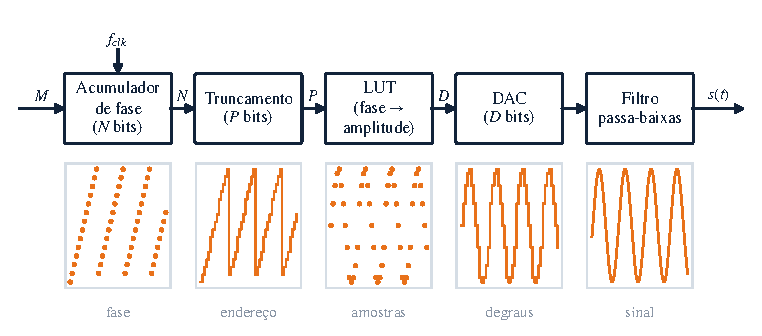
\includegraphics[width=\textwidth]{./figuras/dds_blocos}
	\legend{Fonte~---~Autoria própria.}
\end{figure}

\subsection{Acumulador de fase}

O acumulador de fase é um somador de \(N\)~bits cuja saída é registrada e realimentada. A cada borda do clock, ele soma ao valor atual a palavra de sintonia \(M\), também chamada de \ac{ftw}:
\begin{equation}\label{eq:acumulador}
	\phi[k] = \left(\phi[k-1] + M\right) \bmod 2^{N}.
\end{equation}
O valor \(\phi[k]\) representa a fase do sinal: os \(2^N\) estados do registrador correspondem a uma volta completa, de 0 a \(2\pi\). O estouro natural do somador, que descarta o vai-um, realiza a operação módulo sem nenhuma lógica adicional. Como a fase avança \(M\) estados por clock, uma volta leva \(2^N/M\) clocks, e a frequência de saída é
\begin{equation}\label{eq:fout}
	f_{out} = \frac{M \cdot f_{clk}}{2^{N}}.
\end{equation}

A menor variação de frequência possível, a resolução do gerador, corresponde a \(M = 1\):
\begin{equation}\label{eq:resolucao}
	\Delta f = \frac{f_{clk}}{2^{N}}.
\end{equation}
Com \(N = 32\) e \(f_{clk} = 10\)~MHz, \(\Delta f \approx 2{,}33\)~mHz. Essa resolução fina com um clock fixo é a principal vantagem da \ac{dds} sobre as técnicas baseadas em \ac{pll} \cite{goldberg1999}.

A Figura~\ref{fig:roda_fase} ilustra o acumulador como uma roda: com \(N = 8\), a roda tem 256 estados, e o ponteiro avança \(M = 40\) estados a cada clock. Como 256 não é múltiplo de 40, uma volta leva 6,4 clocks, e as amostras caem em posições diferentes a cada período; ainda assim, o período médio é exatamente o dado pela Equação~(\ref{eq:fout}). Quando \(M\) muda, o acumulador continua a partir da fase em que estava, de modo que a troca de frequência não produz salto de fase. Pelo teorema da amostragem, o passo deve satisfazer \(M < 2^{N-1}\), ou seja, \(f_{out} < f_{clk}/2\); acima disso, o sinal amostrado aparece com frequência \(f_{clk} - f_{out}\), fenômeno conhecido como \eng{aliasing} \cite{oppenheim2010}.

\begin{figure}
	\caption{Roda de fase de um acumulador de 8~bits com \(M = 40\) e tabela de 16 posições: à esquerda, as primeiras posições do ponteiro; à direita, as amostras resultantes.}
	\label{fig:roda_fase}
	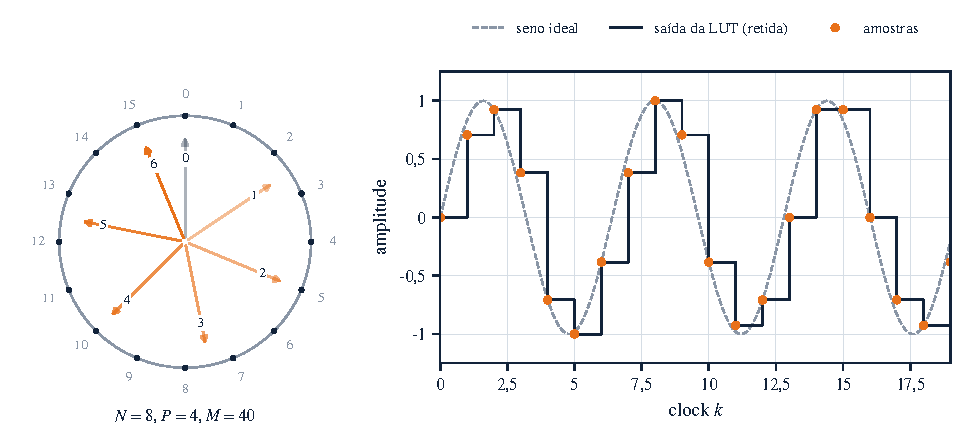
\includegraphics[width=\textwidth]{./figuras/roda_fase}
	\legend{Fonte~---~Autoria própria.}
\end{figure}

\subsection{Conversão de fase em amplitude}

A conversão de fase em amplitude é feita por uma tabela que guarda um período da forma de onda, com \(2^P\) amostras de \(D\)~bits. Para uma senoide em código binário deslocado, o conteúdo da posição \(n\) é
\begin{equation}\label{eq:lut_seno}
	x[n] = \operatorname{round}\!\left(2^{D-1} + \left(2^{D-1}-1\right)\sin\frac{2\pi n}{2^{P}}\right),
\end{equation}
de forma que o zero do sinal corresponde ao código \(2^{D-1}\). Como a tabela pode conter qualquer sequência, a mesma arquitetura gera rampas, pulsos ou formas arbitrárias. Para senoides, há técnicas que reduzem o tamanho da tabela explorando a simetria do seno, guardando apenas um quarto de período, ou que substituem a tabela por aproximações polinomiais ou pelo algoritmo CORDIC \cite{vankka2001}. Neste trabalho a tabela completa é usada, pois a memória do \ac{fpga} é suficiente e a mesma estrutura atende às formas arbitrárias.

A amostra de \(D\)~bits introduz um erro de quantização de amplitude. Para uma senoide de escala completa, considerando o erro como ruído uniforme, a \ac{snr} máxima é \cite{kester2005}
\begin{equation}\label{eq:snr}
	\mathrm{SNR} \approx 6{,}02\,D + 1{,}76~\text{dB},
\end{equation}
que resulta em cerca de 50~dB para \(D = 8\).

\subsection{Truncamento de fase e espúrios}

Uma tabela com \(2^{N}\) posições seria inviável: com \(N = 32\), seriam mais de quatro bilhões de amostras. Por isso, apenas os \(P\)~bits mais significativos da fase endereçam a tabela, e os \(N-P\) bits restantes são descartados. Os bits descartados continuam acumulando, de modo que a frequência média permanece correta, mas a fase usada para endereçar a tabela tem um erro periódico. Esse erro modula a fase do sinal de saída e aparece no espectro como componentes espúrias discretas. No pior caso, a \ac{sfdr}, distância entre a portadora e o maior espúrio, é aproximadamente \cites{nicholas1987,vankka2001}
\begin{equation}\label{eq:sfdr}
	\mathrm{SFDR} \approx 6{,}02\,P~\text{dBc}.
\end{equation}

A Figura~\ref{fig:espectros}(a) mostra o espectro das amostras de um \ac{dds} com \(N = 32\), \(P = 10\) e \(D = 8\), os parâmetros deste trabalho, obtido por simulação numérica com \ac{fft} de \(2^{16}\) pontos e janela de Blackman. O maior espúrio fica 60,1~dB abaixo da portadora, em acordo com a Equação~(\ref{eq:sfdr}), que prevê 60,2~dB para \(P = 10\). O piso de ruído, abaixo dos espúrios, vem da quantização de amplitude.

\begin{figure}
	\caption{(a) Espectro das amostras de um \acs{dds} com \(N = 32\), \(P = 10\) e \(D = 8\), obtido por simulação numérica; (b) saída de um \acs{dac} com retenção de ordem zero: imagens em torno dos múltiplos de \(f_{clk}\), envoltória sinc e efeito do filtro de reconstrução usado neste trabalho.}
	\label{fig:espectros}
	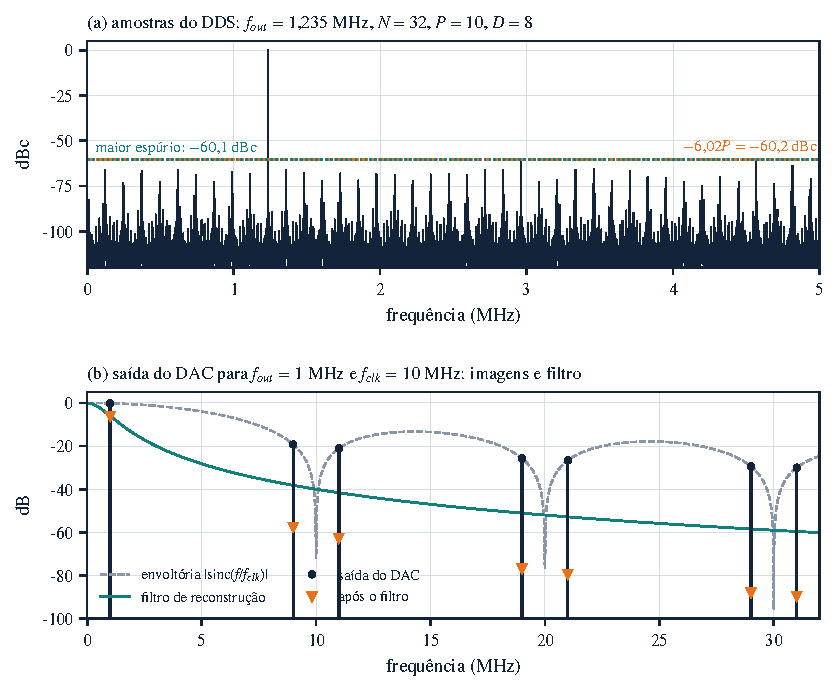
\includegraphics[width=\textwidth]{./figuras/espectros}
	\legend{Fonte~---~Autoria própria.}
\end{figure}

\subsection{Conversão digital-analógica e reconstrução}

O \ac{dac} mantém cada amostra na saída durante um período de clock, comportando-se como um \ac{zoh}. O sinal resultante é uma escada, cujo espectro contém, além da componente em \(f_{out}\), imagens em \(k f_{clk} \pm f_{out}\), para todo inteiro \(k \geq 1\). Todas as componentes são ponderadas pela resposta do retentor \cites{kester2005,oppenheim2010}:
\begin{equation}\label{eq:zoh}
	\left|H_{\mathrm{ZOH}}(f)\right| = \left|\frac{\sin(\pi f/f_{clk})}{\pi f/f_{clk}}\right|.
\end{equation}
A Equação~(\ref{eq:zoh}) mostra que a própria componente desejada é atenuada à medida que se aproxima de \(f_{clk}/2\): em \(f_{out} = f_{clk}/2\), a perda é de 3,9~dB. Para frequências bem abaixo de \(f_{clk}\), a atenuação é desprezível.

O filtro de reconstrução é um passa-baixas que deixa passar \(f_{out}\) e atenua as imagens. Quanto mais próximo \(f_{out}\) estiver de \(f_{clk}/2\), mais próxima a primeira imagem fica da banda útil e mais seletivo o filtro precisa ser. A Figura~\ref{fig:espectros}(b) mostra esse efeito para \(f_{out} = 1\)~MHz e \(f_{clk} = 10\)~MHz, com o filtro de segunda ordem usado neste trabalho.

\section{Dispositivos lógicos programáveis}

\subsection{FPGA e a família Cyclone IV E}

Um \ac{fpga} é um circuito integrado cuja função lógica é definida após a fabricação, por configuração. Na família Cyclone IV E, da Intel, o recurso básico é o \ac{le}, composto por uma tabela de quatro entradas, que implementa qualquer função combinacional dessas entradas, e por um registrador programável. Além dos \acp{le}, o dispositivo oferece blocos de memória M9K, de 9\,216~bits cada, que podem ser configurados como \ac{rom} ou como \ac{ram} de uma ou duas portas; multiplicadores dedicados de \(18 \times 18\)~bits, que também operam como dois de \(9 \times 9\); e \acp{pll}, que geram clocks com frequência múltipla ou submúltipla da referência \cite{intel2016cyclone}.

A placa DE2-115, da Terasic, usa o EP4CE115F29C7, com 114\,480 \acp{le}, 432 blocos M9K (3\,981\,312~bits de memória), 266 multiplicadores de \(18 \times 18\)~bits e quatro \acp{pll}. A placa oferece um oscilador de 50~MHz, botões com circuito de \eng{debounce}, \eng{LEDs}, um conector de expansão de 40 pinos com \ac{gpio} e um gravador USB-Blaster integrado, acessível pela porta \ac{usb} \cite{terasic2010}.

\subsection{VHDL e fluxo de projeto}

O \ac{vhdl} é uma linguagem de descrição de hardware padronizada pelo IEEE \cite{ieee2009vhdl}. Um projeto em \ac{vhdl} é organizado em entidades, que declaram as portas de um bloco, e arquiteturas, que descrevem seu comportamento ou sua estrutura. Uma arquitetura estrutural instancia outras entidades e as liga por sinais, o que permite construir o sistema de forma hierárquica, com cada bloco encapsulado atrás de sua interface \cite{pedroni2010}.

O mesmo código \ac{vhdl} tem dois usos. Na síntese, uma ferramenta como o Quartus Prime traduz a descrição em \acp{le}, memórias e conexões do \ac{fpga} e verifica se os caminhos entre registradores cumprem os requisitos de tempo do clock. Na simulação, um simulador como o GHDL executa a descrição em um computador, dentro de um \eng{testbench}: uma entidade sem portas que gera os estímulos, observa as saídas e, quando é auto-verificável, compara o resultado com um modelo de referência \cites{pedroni2010,ghdl2025}.

Funções comuns são oferecidas pelo fabricante como blocos de \ac{ip}, configurados por assistentes. Neste trabalho são usados o \cod{altsyncram}, que implementa memórias nos blocos M9K \cite{intel2018ram}, e o \cod{altpll}, que configura um \ac{pll} \cite{intel2017pll}. Ambos têm modelos de simulação em \ac{vhdl} distribuídos com o Quartus.

\subsection{JTAG e Virtual JTAG}

O padrão IEEE 1149.1, conhecido como \ac{jtag}, define uma \ac{tap} serial, com os sinais TCK, TMS, TDI e TDO, controlada por uma máquina de estados. Duas sequências de estados são usadas para acessar o dispositivo: a do registrador de instrução (IR), que escolhe qual registrador de dados será acessado, e a do registrador de dados (DR). No acesso ao DR, o estado Capture-DR carrega um valor no registrador; o Shift-DR desloca os bits, um por clock, entrando por TDI e saindo por TDO; e o Update-DR aplica o valor deslocado \cite{ieee2013jtag}.

Nos \acp{fpga} da Intel, a mesma porta \ac{jtag} usada para a gravação pode ser compartilhada com a lógica do usuário. O bloco Virtual \ac{jtag} cria uma \ac{tap} virtual: ele entrega ao projeto o clock \cod{tck}, o bit \cod{tdi}, a instrução atual (\cod{ir\_in}) e sinais que indicam os estados Capture-DR, Shift-DR e Update-DR, e recebe de volta o bit \cod{tdo}. No computador, o programa \cod{quartus\_stp} oferece comandos Tcl para deslocar valores nos registradores IR e DR virtuais, através do USB-Blaster \cite{intel2018vjtag}.

\subsection{Domínios de clock e metaestabilidade}\label{sec:cdc}

Quando um sinal muda próximo à borda do clock de um \eng{flip-flop}, violando os tempos de \eng{setup} ou de \eng{hold}, a saída do \eng{flip-flop} pode ficar por um tempo indeterminado em um nível intermediário, estado chamado de metaestável. Isso ocorre sempre que um sinal passa de um domínio de clock para outro, sem relação de fase entre eles. A solução usual para um sinal de um bit é o sincronizador: dois ou três \eng{flip-flops} em série no domínio de destino, que dão tempo para a metaestabilidade se resolver antes do sinal ser usado. O tempo médio entre falhas cresce exponencialmente com o tempo disponível para essa resolução \cite{ginosar2011}.

Um barramento de vários bits não pode ser sincronizado bit a bit, pois cada bit pode ser capturado em uma borda diferente, resultando em uma palavra que nunca existiu. Uma técnica segura é manter os dados parados no domínio de origem e sinalizar a novidade por um único bit, que muda de nível a cada transferência (\eng{toggle}). Apenas esse bit passa pelo sincronizador; quando sua mudança é detectada no destino, os dados já estão estáveis e podem ser copiados \cites{cummings2008,ginosar2011}.

\section{Circuitos analógicos de saída}

\subsection{O conversor DAC0800}

O DAC0800 é um conversor digital-analógico multiplicador de 8~bits com saídas complementares em corrente, \(I_{OUT}\) e \(\overline{I_{OUT}}\). Uma corrente de referência \(I_{REF}\), definida por uma tensão \(V_{REF}\) e um resistor \(R_{REF}\), é dividida por uma rede R-2R. Cada bit da entrada dirige sua parcela para uma das duas saídas, de modo que \cite{ti2013}
\begin{equation}\label{eq:dac0800}
	I_{REF} = \frac{V_{REF}}{R_{REF}}, \qquad I_{OUT} = I_{REF}\,\frac{n}{256}, \qquad I_{OUT} + \overline{I_{OUT}} = I_{FS} = I_{REF}\,\frac{255}{256},
\end{equation}
em que \(n\) é o código de entrada. O tempo de acomodação típico é de 100~ns, e o limiar das entradas lógicas é ajustável por um pino, o que permite a ligação direta com lógica de 3,3~V. O conversor não tem registrador de entrada: a saída acompanha os bits da entrada a todo instante.

\subsection{Conversão corrente-tensão}

A corrente do \ac{dac} é convertida em tensão por amplificadores operacionais. Com um amplificador de diferenças, as duas saídas complementares podem ser aproveitadas: a tensão de saída é proporcional a \(I_{OUT} - \overline{I_{OUT}}\), o que dobra a excursão em relação ao uso de uma só saída e produz um sinal simétrico em torno de zero \cites{ti2013,sedra2015}.

\subsection{Filtro Sallen-Key}

O filtro Sallen-Key é uma topologia ativa de segunda ordem com um único amplificador \cite{sallen1955}. Na versão passa-baixas de ganho unitário, com resistores \(R_1\) e \(R_2\) em série na entrada e capacitores \(C_1\), na realimentação, e \(C_2\), para o terra, a frequência natural e o fator de qualidade são \cite{sedra2015}
\begin{equation}\label{eq:sallen_key}
	f_0 = \frac{1}{2\pi\sqrt{R_1 R_2 C_1 C_2}}, \qquad Q = \frac{\sqrt{R_1 R_2 C_1 C_2}}{C_2\,(R_1 + R_2)}.
\end{equation}
Com resistores iguais e capacitores iguais, \(Q = 0{,}5\): o filtro tem dois polos reais coincidentes em \(f_0\), sem sobressinal na resposta ao degrau, e a atenuação de 3~dB ocorre em \(f_0\sqrt{\sqrt{2}-1} \approx 0{,}64\,f_0\).
